\section{Prepositional Phrase Attachment}\label{ppa}
Prepositional phrases (PPs)   express crucial information that  information extraction  methods need to extract.
 % comprehensively extract facts. 
 However, PPs are a major source of  syntactic  ambiguity. In this paper, we propose to use semantic knowledge to  improve PP attachment disambiguation. 
 PPs such as  ``in", ``at", and ``for" express details about the  \textit{where, when,} and \textit{why}  of  relations and events. PPs   also state  attributes of nouns. 

\begin{figure}[t]

\centering

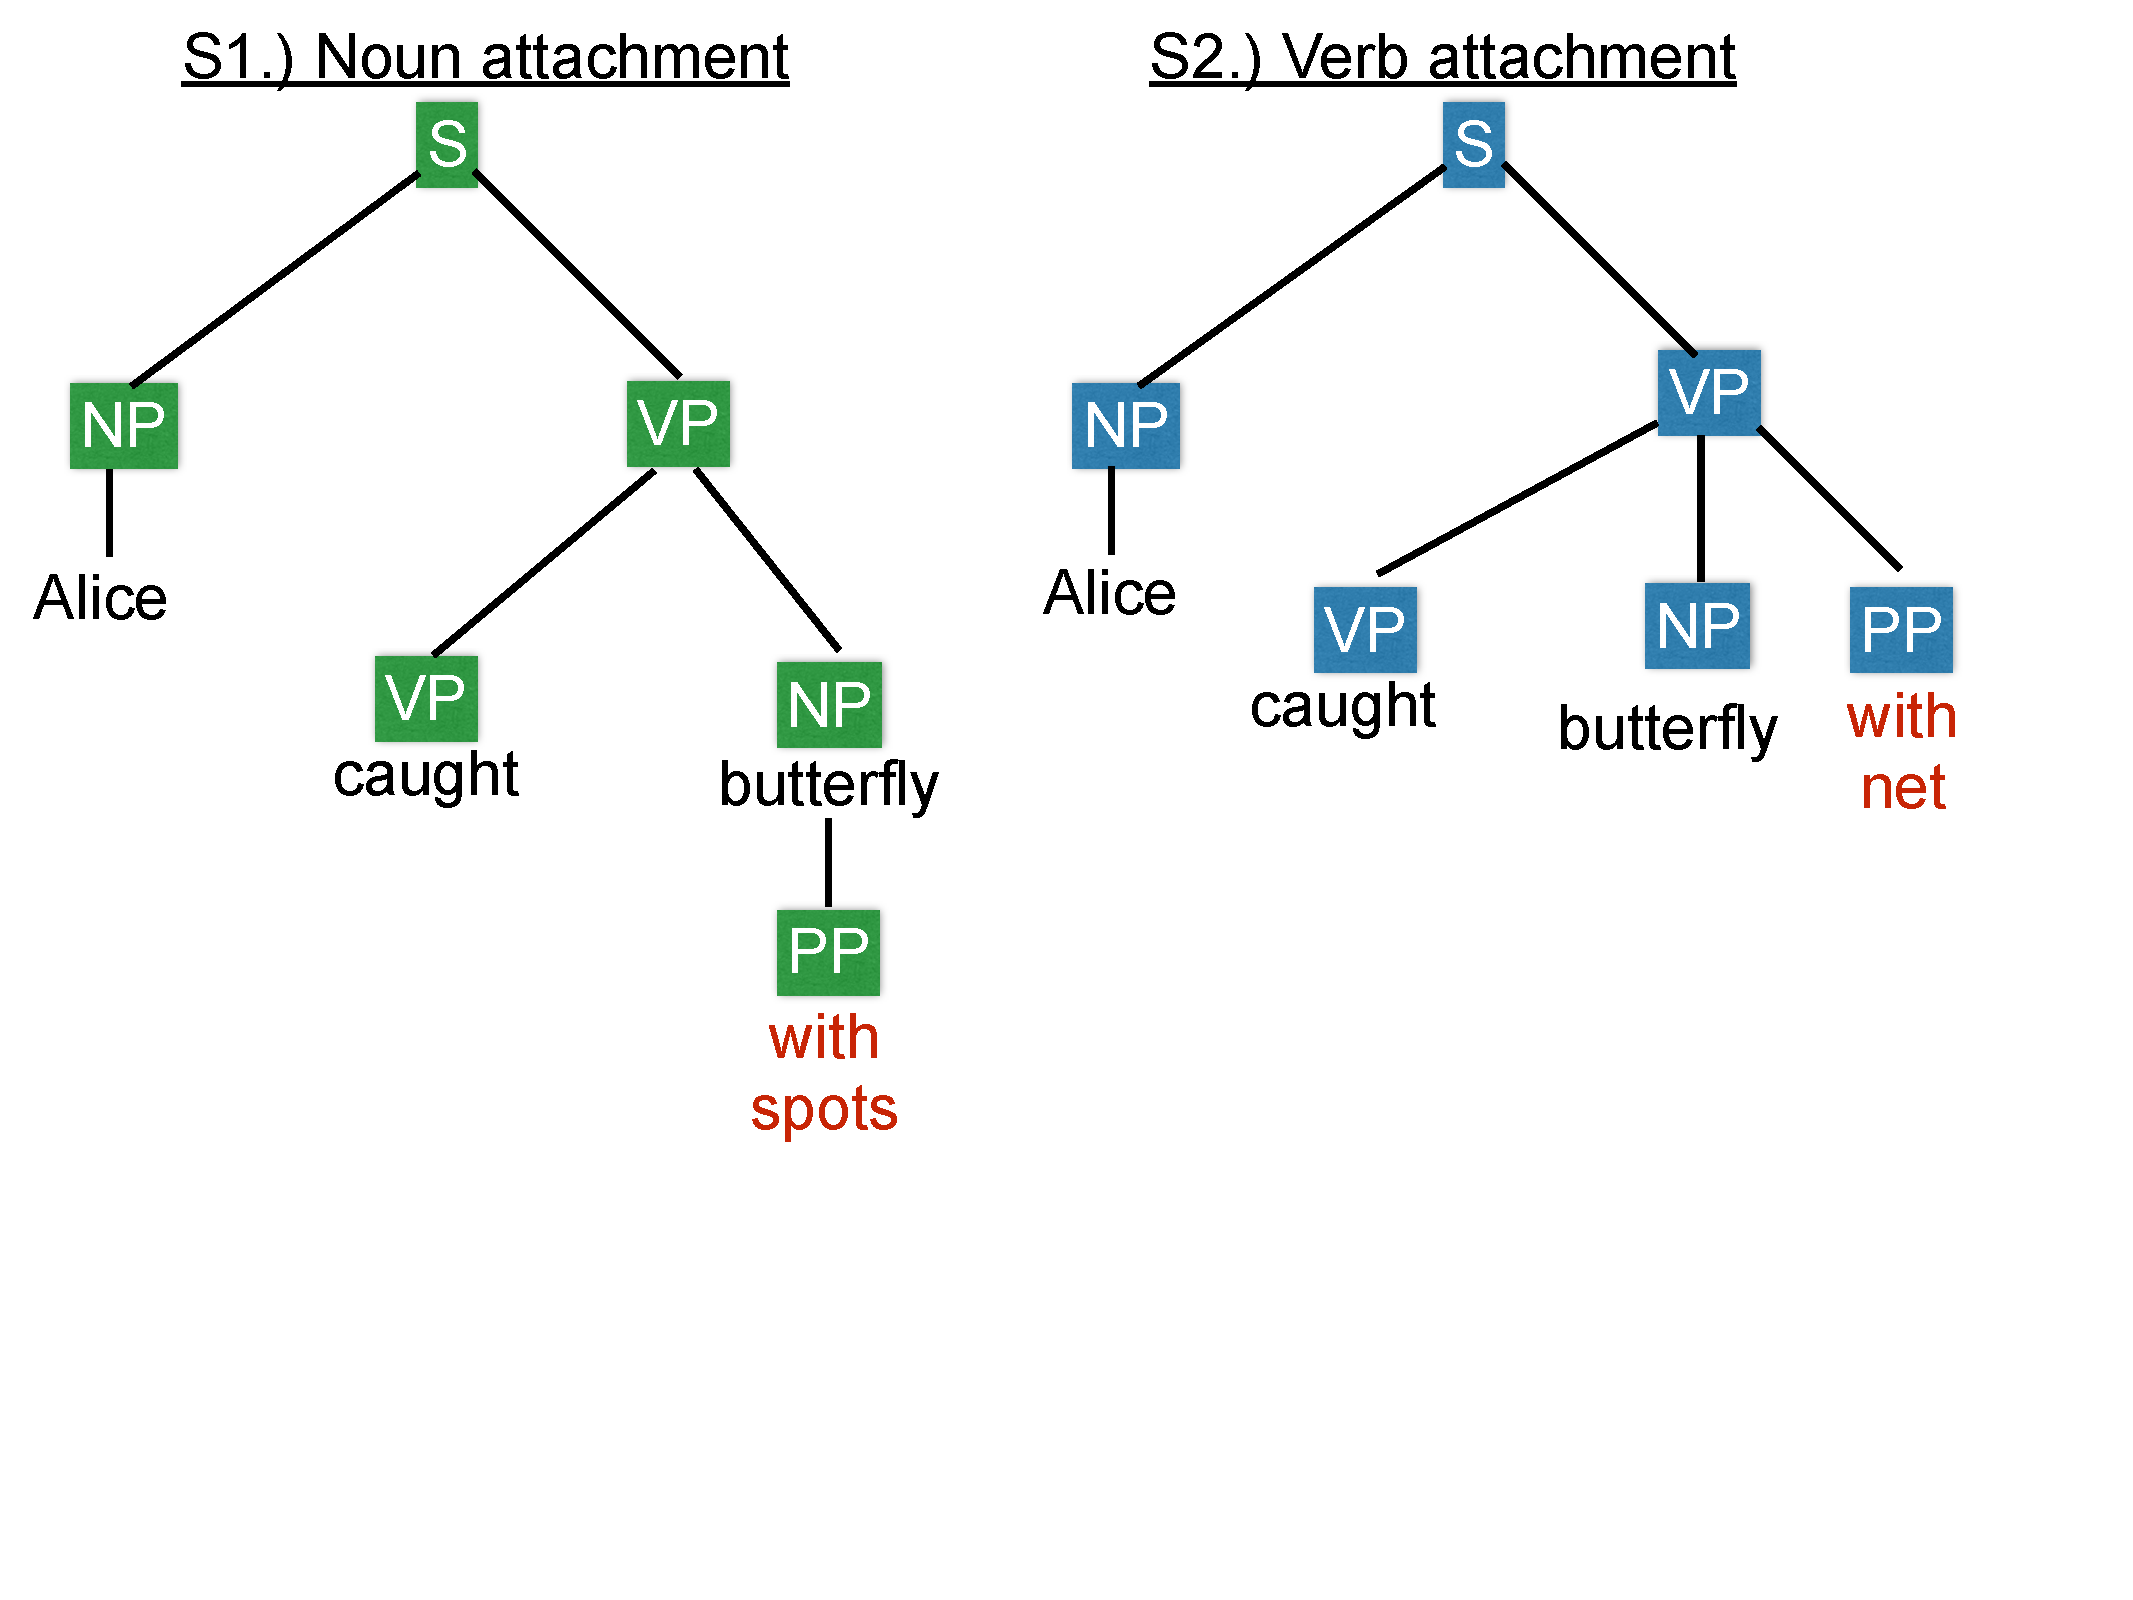
\includegraphics[width=1\columnwidth] {trees2.pdf}
\vspace*{-2.6cm}
\caption{Parse trees where the prepositional phrase (PP) attaches to the noun, and to the verb.}
%The only difference in the parse trees are the PP attachment sites, resulting in trees of different structures.}
%and hence the sentence structures are different. } 

\label{fig:deptrees}

\end{figure}



 As an example, consider the following sentences: \textit{ S1.) Alice caught the butterfly with the spots. S2.) Alice caught the butterfly with the net. }  S1 and S2 are syntactically different, this is evident from their corresponding parse trees in Figure \ref{fig:deptrees}. Specifically,  S1 and S2  differ in where their PPs attach. In  S1,  the butterfly has spots and therefore  the PP, ``with the spots'', attaches to the \textit{noun}. For relation extraction, we  obtain a \textit{binary} relation of the form:  
 $\langle$Alice$\rangle$  caught $\langle$butterfly with  spots$\rangle$.
However, in S2, the net is the instrument used for catching and therefore  the PP,  ``with the net", attaches to the \textit{verb}.  For relation extraction, we get a \textit{ternary} extraction of the form:
%\begin{itemize}
%\item[]
 $\langle$Alice$\rangle$  caught $\langle$butterfly$\rangle$ with $\langle$net$\rangle$.
%\item[] $\langle$The government$\rangle$  discovered $\langle$irregularities$\rangle$ in $\langle$June$\rangle$
%\end{itemize
 
The PP attachment problem is often defined as follows: given a PP occurring within a  sentence where there are multiple possible attachment sites for the PP, choose the most plausible attachment site. 
%Notice that in the examples we have given so far, there were only two possible attachment sites, the noun and the verb.
% as shown in Figure \ref{fig:deptrees} with a parse tree corresponding to each type.
 In the literature,  prior work going as far back as \cite{BrillR94,Ratnaparkhi1994,Collins95} has  focused on the  language pattern that causes most PP ambiguities, which is the  4-word sequence: $\{v, n1, p, n2\}$ (e.g., $\{${\em caught, butterfly, with, spots}$\}$). The task is  to   determine if  the prepositional phrase $(p,n2)$  attaches to  the verb $v$ or to the first noun $n1$.
Following common practice,  we focus on  PPs occurring as $\{v,n1,p,n2\}$ quadruples ---  we shall refer to these as  \textit{PP quads}. 

The approach we present here differs from prior work in two main ways. First, we make extensive use of semantic knowledge about nouns, verbs, prepositions, pairs of nouns, and  the discourse context in which a PP quad occurs. Table \ref{tab:knowledge}  summarizes the types of  knowledge we considered in our work. Second, in training our model, we rely on both labeled and unlabeled data, employing an expectation maximization (EM) algorithm \cite{Dempster77maximumlikelihood}. 


\begin{table}[h]
\centering
\small{
   \begin{tabular}{|p{1.8cm}|p{4.9cm}|}
     % \hline
   %&  {\bf Definition \& Example(s)}  \\
     \hline
    % \newline -receive(agent, patient, source) \\
     % \newline -isA(tea,beverage)\\
     Relations &  Noun-Noun binary relations  \newline \textit{ (Paris, located in, France)} \newline \textit{(net, caught, butterfly)}\\
     \hline
     Nouns &  Noun semantic categories \newline \textit{(butterfly, isA, animal)}  \\
     \hline
     Verbs & Verb roles \newline  \textit{caught(agent, patient, instrument)} \\
     \hline
     % \newline -(fork, used for, eating) \\
     Prepositions& Preposition  definitions \newline  
     \textit{ f(for)= used for, has purpose, ...}  
     \newline \textit{f(with)= has, contains, ...}  \\
     \hline
     Discourse &  Context \newline  $n0 \in \{n0, v, n1, p, n2\}$\\
     \hline
   \end{tabular}
   \caption{Types of background   
   knowledge used in this paper to determine PP attachment.}
     \label{tab:knowledge}
     }      
   \end{table}   
   

\begin{figure}[t]
%
\centering
%
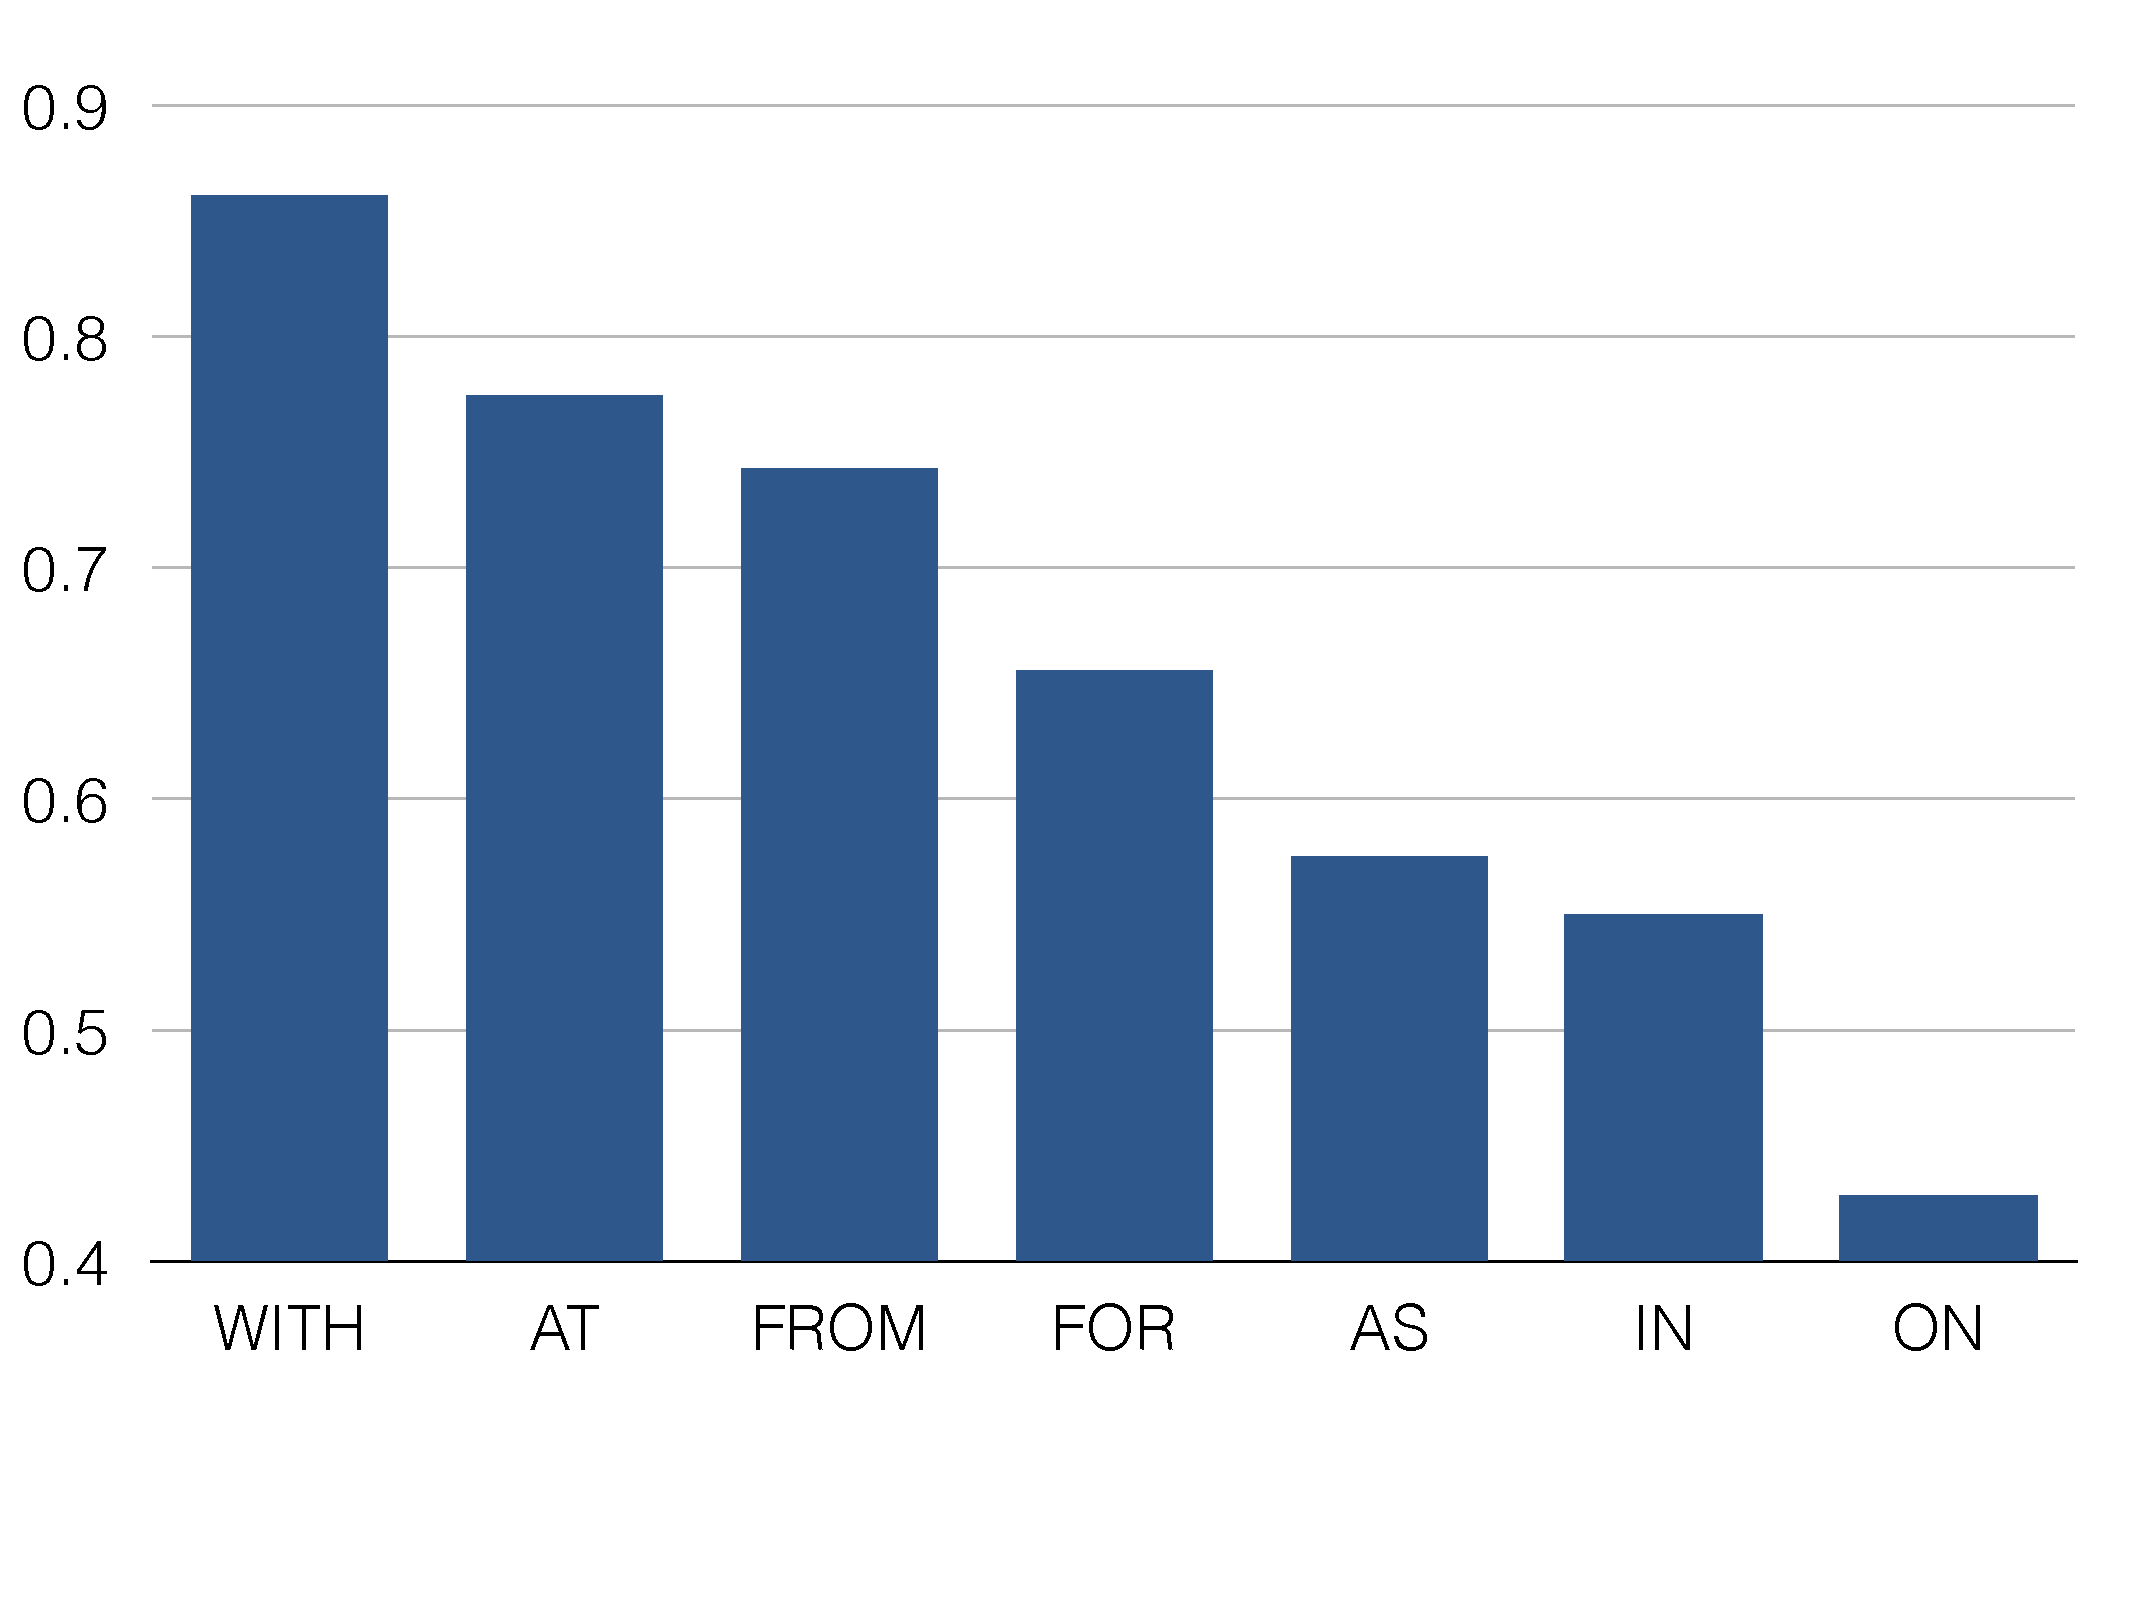
\includegraphics[width=0.80\columnwidth] {mainresults-0.pdf}
\vspace*{-0.8cm}
\caption{Dependency parser PP attachment accuracy for various frequent prepositions.}
% The only difference in the parse trees are the PP attachment sites, resulting in trees of different structures.}
% and hence the sentence structures are different. } 
%
\label{fig:parser}
%
\end{figure}  

                